\section{Lecture: 16/10/2024}

\begin{example}
	Let $R=\Z[\sqrt{-3}]$ and $x=1+\sqrt{-3}$. 
	\begin{enumerate}
		\item $x$ is irreducible. 
	If $x=\alpha\beta$ for some $\alpha,\beta\in R$, then 
	\[
 4=\norm(x)=\norm(\alpha)\norm(\beta).
 \]
 Thus $\norm(\alpha)\in\{1,2,4\}$. 
	Write $\alpha=a+b\sqrt{-3}$ for some $a,b\in\Z$. 
	If $\norm(\alpha)=a^2+3b^2=2$, then $b=0$ and hence
	$a^2=2$, a contradiction. If $\norm(\alpha)=1$, then $\alpha\in\mathcal{U}(R)$.
	If $\norm(\alpha)=4$, then $\norm(\beta)=1$ and $\beta\in\mathcal{U}(R)$. 
%
%	If $\norm(\alpha)=2$, then $a^2+3b^2=2$ and then $a$ and $b$
%	both have the same parity. 
%	
%	If both $a$ and $b$ are even, say $a=2k$ and $b=2l$ for
%	some $k,l\in\Z$, then 
%	\[
%	2=a^2+3b^2=4k^2+12l^2
%	\]
%	is divisible by 4, a contradiction.  
%	
%	If both $a$ and $b$ are odd, say $a=2k+1$ and $b=2l+1$ for some $k,l\in\Z$, then
%	\[
%	2=a^2+3b^2=4k^2+4k+12l^2+12l+4
%	\]
%	is divisible by 4, a contradiction. 
		\item $x$ is not prime. Note that 
  \[
  (1+\sqrt{-3})(1-\sqrt{-3})=4,
  \]
  then 
		$x$ divides $4=2\cdot 2$. But $1+\sqrt{-3}\nmid 2$, as 
		\[
		(a-3b)+(a+b)\sqrt{-3}=(1+\sqrt{-3})(a+b\sqrt{-3})=2
		\]
		implies that $a-3b=2$ and $a+b=0$, which yields 
		$a=1/2\not\in\Z$, a contradiction.
	\end{enumerate}
\end{example}

\begin{exercise}
	Let $R=\Z[\sqrt{-5}]$. 
	\begin{enumerate}
		\item Prove that $1+\sqrt{-5}$ and $1-\sqrt{-5}$ are irreducible in $R$. 
		\item Prove that $2,3,1+\sqrt{-5}$ and $1-\sqrt{-5}$ are not associate in $R$.
	\end{enumerate}
\end{exercise}

\begin{exercise}
	Let $R=\Z[\sqrt{5}]$. 
	Prove that $1+\sqrt{5}$ is irreducible and not prime in $R$. 	
\end{exercise}

\begin{definition}
	Let $R$ be an integral domain. Then $R$ is \emph{principal} 
	(or a principal ideal domain) if
	every ideal $I$ of $R$ is of the form $I=(x)$ for some $x\in R$.   
\end{definition}

An ideal $I$ of the form $I=(x)$ for some $x$ is called a \emph{principal ideal}. 

The rings $\Z$ and $\R[X]$ are both principal. 

\begin{example}
	The ring $\Z[X]$ is not principal. For example, the ideal
	$I=(2,X)$ is not principal. 
	
	First note that $I\ne\Z[X]$. In fact, if $I=\Z[X]$, then 
	$1=2f(X)+Xg(X)$ for some polynomials $f(X),g(X)\in\Z[X]$. Then 
	$1=2f(0)$, which implies that $-1/2=f(0)\in\Z$, a contradiction. 
	
	If $I=(h(X))$ for some $h(X)\in\Z[X]$, then $2=h(X)g(X)$ for some $g(X)\in\Z[X]$. This
	implies that $\deg(h(X))=0$, so $h(X)=h(1)\in\Z$. In particular, $2=h(1)g(1)$ and hence
	$h(1)\in\{-1,1,2,2\}$. Since $I\ne\Z[X]$, it follows that $h(X)=h(1)\not\in\{-1,1\}$. Now      
	$X=h(X)f(X)$ for some $f(X)\in\Z[X]$. In particular, $\deg(f(X))=1$, so
	we may assume that $f(X)=a_0+a_1X$ for $a_0,a_1\in\Z$ and $a_1\ne 0$. 	
	It follows that 
	\[
	X=\pm 2f(X)=\pm2(a_0+a_1X)
	\]
	and therefore $\pm1/2=a_1\in\Z$, a contradiction.
\end{example}

\begin{exercise}
\label{xca:principal=>noetherian}
    Let $R$ be a principal domain. Prove that $R$ is noetherian.
\end{exercise}

\begin{example}
	Let $R=\Z[\sqrt{-5}]$.  
	The ideal $I=(2,1+\sqrt{-5})$ is not principal, so $R$ is not principal. 
	
	We first note that $I\ne R$. If not, there exist $x,y,u,v\in\Z$ such that 
	\[
	1=2(x+y\sqrt{-5})+(1+\sqrt{-5})(u+v\sqrt{-5})=(2x+u-5v)+\sqrt{-5}(2y+u+v).
	\]
	This implies that $1=2x+u-5v$ and $0=2y+u+v$. These formulas imply that
	\[
    1=2(x+y+u-2v),
    \]
    a contradiction because $x+y+u-2v\in\Z$. 
	
	Now assume that $I=(\alpha)$ for some $\alpha$. Then $\alpha\mid 2$ and $\alpha\mid 1+\sqrt{-5}$. Then
	$\norm(\alpha)\mid 4$ and $\norm(\alpha)\mid 6$, because $\norm(2)=4$ and $\norm(1+\sqrt{-5})=6$. 
	Thus $\norm(\alpha)\in\{1,2\}$. If we write
	$\alpha=a+b\sqrt{-5}$ for $a,b\in\Z$, then it follows that 
	$a^2+5b^2=\norm(\alpha)$. Clearly, $\norm(\alpha)\ne 2$, as $a^2=2$ has no solution in $\Z$.
	Now $\norm(\alpha)= 1$ implies that $\alpha\in\mathcal{U}(R)$ and hence 
	$I=R$, a contradiction.   
\end{example}

Sometimes primes and irreducibles coincide. 

\begin{proposition}
\label{pro:PID:irreducible=prime}
	Let $R$ be a principal domain and $x\in R$. 
	Then $x$ is irreducible if and only if $x$ is prime. 	
\end{proposition}

\begin{proof}
	We only need to prove that if $x$ is irreducible, then $x$ is prime. Let us
	assume that $x\mid yz$. Let $I=(x,y)$. Since $R$ is principal, $I=(a)$ for some $a\in R$. In particular, $x=ab$ for some $b\in R$. Since $x$ is irreducible, $a\in\mathcal{U}(R)$ or
	$b\in\mathcal{U}(R)$. If $a\in\mathcal{U}(R)$, then $I=R$ and hence 
	$1=xr+ys$ for some $r,s\in R$. Thus
	\[
	z=z1=z(xr+ys)=zxr+zys
	\]
	and therefore $x\mid z$. If $b\in\mathcal{U}(R)$, then $x$ and $a$ are associate
	in $R$. Thus $I=(x)=(a)$ and hence $xt=y$ for some $t\in R$, that is $x\mid y$.  
\end{proof}

In the integers primes and irreducible coincide. This happens 
because $\Z$ is a principal domain.

\begin{example}
	Since $\Z[\sqrt{-3}]$ have irreducible elements that are not prime, 
	$\Z[\sqrt{-3}]$ is not a principal domain.
\end{example}

\begin{definition}
	Let $R$ be an integral domain. We say that $R$ is an \emph{euclidean domain}
	if there exists a map $\varphi\colon R\setminus\{0\}\to\Z_{\geq0}$ such that
	for every $x,y\in R$ with $y\ne 0$ there exist $q,r\in R$ such that 
	$x=qy+r$, where $r=0$ or $\varphi(r)<\varphi(y)$. 
\end{definition}

Note that in the definition of euclidean domains, we do not ask for the uniqueness 
of the quotient and the remainder. In fact, 
we will meet important examples of euclidean domains where uniqueness
in the division algorithm is not achieved. 

\begin{example}
	$\Z$ is a euclidean domain with $\varphi(x)=|x|$.
\end{example}

Do we have uniqueness in the previous example? 	

\begin{example}
	$\R[X]$ is a euclidean domain with $\varphi(f(X))=\deg(f(X))$. 	
\end{example}

The previous examples suggest why for the definition of a euclidean domain one needs to  
consider a map $\varphi\colon R\setminus\{0\}\to\Z_{\geq0}$. 

\begin{example}
	Let $R=\Z[i]$. Then $R$ is a euclidean domain with $\varphi(\alpha)=\norm(\alpha)$. Let 
	Let $\alpha,\beta\in\Z[i]$ and assume that $\beta\ne0$. 
	We want to find Gauss integers $\gamma,\delta\in\Z[i]$ such that 
	\[
        \alpha=\beta\delta+\gamma 
	\]
	and
	$\varphi(\gamma)<\varphi(\beta)$. Note that every complex
	number $z\in\C$ can be written as $z=\xi+\eta$, where $\xi\in\Z[i]$ and $\varphi(\eta)<1$. Indeed, this
	follows from the fact that 
	$\C$ is covered by open unit disks of radius one and centers in Gauss integers, see the following figure:
	%Figure \ref{fig:covering}. 

	\begin{figure}[ht]
		\centering
	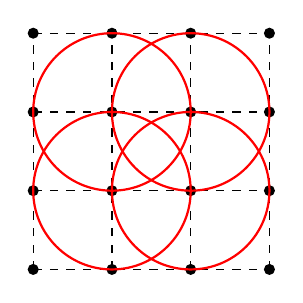
\begin{tikzpicture} 
\draw[dashed] (0,0) grid (3,3); 
\foreach \i in {0,...,3}     
\foreach \j in {0,...,3}         
\fill (\i,\j) circle (2pt);  
\draw[red,thick](1,1) circle (1);
\draw[red,thick](2,1) circle (1);
\draw[red,thick](1,2) circle (1);
\draw[red,thick](2,2) circle (1);
\end{tikzpicture}
%\caption{$\C$ is covered by open unit disks of radius one and centers in $\Z[i]$.}
\label{fig:covering}
\end{figure}
	
	Now let $\alpha=a+ib$ and $\beta=c+id$, where $a,b,c,d\in\Z$.  
	Write 
	\[
	\frac{\alpha}{\beta}=\frac{a+ib}{c+id}=r+is
	\]
	for some $r,s\in\Q$. We don't need to compute $r$ and $s$ explicitly! 
        Let $m,n\in\Z$ be such that $|r-m|\leq 1/2$ and 
	$|s-n|\leq 1/2$. If $\delta=m+in$ and $\gamma=\alpha-\beta\delta$, then 
	$\gamma\in R$, $\delta\in R$ and $\alpha=\beta\delta+\gamma$. If $\gamma\ne0$, then
	\begin{align*}
	\varphi(\gamma)&=\varphi\left(\beta\left(\frac{\alpha}{\beta}-\delta\right)\right)
	=\varphi(\beta)\varphi\left(\frac{\alpha}{\beta}-\delta\right)\\
	&=\varphi(\beta)\varphi((r-m)+i(s-n))
	=\varphi(\beta)((r-m)^2+(s-n)^2)\\
	&\leq\varphi(\beta)(1/4+1/4)\\
	&<\varphi(\beta).
	\end{align*}	
\end{example}



In $\Z[i]$ the division algorithm does not have uniqueness. In fact, 
if $\alpha,\beta\in\Z[i]$ and $\alpha=\beta\delta+\gamma$ 
for some $\delta,\gamma\in\Z[i]$, 
then there are up to four possibilities 
for the remainder $\gamma$.

\begin{example}
	Let $R=\Z[i]$ and 
	$\alpha=-1+i$ and $\beta=1+2i$. Let $I=(\beta)$ be the ideal of $R$ generated by $\beta$. 
	First, note that
	\[
	I=(\beta)=(1+2i)R=(1+2i)\Z+(1+2i)\Z i=(1+2i)\Z+(-2+i)\Z.
	\]  
	This allows us to draw the lattice of elements of $I$, 
	that is the lattice formed by the multiples of $\beta$, see Figure~\ref{fig:Z[i]}. 
	Since $\alpha-\gamma\in I=(\beta)$, there are at most four possibilities for writing
	the division algorithm. 
	In our particular example, we find three possible cases:
	\begin{enumerate}
		\item If $\alpha-\gamma=\beta_0$, where $0=\beta_0=\beta 0$, 
			then $\gamma=\alpha=-1+i$ and 
				\[
				-1+i=(1+2i)0+(-1+i)
				\]
				with $\norm(-1+i)=2<\norm(\beta)=5$. 
		\item If $\alpha-\gamma=\beta_1$, where $-2+i=\beta_1=\beta i$, then 
			$\gamma=1$ and 
			\[
			-1+i=(1+2i)i+(-1)
			\]
			with $\norm(-1)=1<\norm(\beta)=5$. 
		\item If $\alpha-\gamma=\beta_2$, where $-1+3i=\beta_2=\beta (1+i)$, 
			then $\gamma=2i$ and  
			\[
			-1+i=(1+2i)(1+i)+(-2i)
			\]
			and $\norm(-2i)=4<\norm(\beta)=5$. 
	\end{enumerate}
%	We note that the case $\alpha-\gamma=\beta$ yields $\gamma=-2-i$ and thus
%	$\norm(\gamma)=\norm(\beta)=5$.  
\end{example}

\begin{figure}
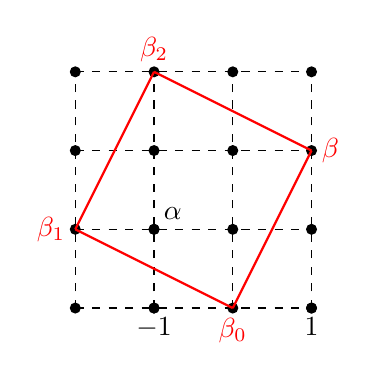
\begin{tikzpicture} 
\draw[dashed] (0,0) grid (3,3); 
\foreach \i in {0,...,3}     
\foreach \j in {0,...,3}         
\fill (\i,\j) circle (2pt);  
\draw[red,thick] 
(2,0)--(0,1) node[anchor=east] {$\beta_1$} 
(0,1)--(1,3) node[anchor=south] {$\beta_2$} 
(1,3)--(3,2) node[anchor=west] {$\beta$} 
(3,2)--(2,0) node[anchor=north] {$\beta_0$} ;
\fill (1,1) circle (2pt) node[anchor=south west] {$\alpha$}  ;
\fill (1,0) circle (2pt) node[anchor=north] {$-1$}  ;
\fill (3,0) circle (2pt) node[anchor=north] {$1$}  ;
\end{tikzpicture}
\caption{Division algorithm in $\Z[i]$.}
\label{fig:Z[i]}
\end{figure}

We know that $\Z$ and $\R[X]$ are both principal. The proofs 
are very similar, as both use the division algorithm essentially in the same way. 
The following result takes advantage of this fact. 

\begin{proposition}
	Let $R$ be a euclidean domain. Then $R$ is principal.	
\end{proposition}

\begin{proof}
	Let $I$ be an ideal of $R$. If $I=\{0\}$, then $I=(0)$ and hence 
	it is principal. So we may
	assume that $I\ne\{0\}$. Let $y\in I\setminus\{0\}$ be such that
	$\varphi(y)$ is minimal. We claim that $I=(y)$. 
	If $z\in I$, then $z=yq+r$, where $r=0$ or $\varphi(r)<\varphi(y)$. 
	The minimality of $\varphi(y)$ implies that $r=0$. Thus $z=yq\in (y)$ and 
	it follows that 
	$I=(y)$. 
\end{proof}

\begin{example}\
	Since $\Z[i]$ is euclidean, it is principal.
\end{example}
 
\begin{example}
	The rings $\Z[\sqrt{-5}]$ and $\Z[\sqrt{-3}]$ are
	not euclidean. Why?
\end{example}

The ring $\Z[\frac{1+\sqrt{-19}}{2}]$ is an 
example of a ring that is principal and not euclidean. We will not prove this
fact in these notes. For a proof 
see \cite{MR967349}, \cite{MR3665445} or \cite{MR314831}.

\begin{definition}
	Let $R$ be an integral domain. Then $R$ is a 
	\emph{unique factorization domain}
	if the following statements hold:
	\begin{enumerate}
	\item Each $x\in R\setminus\{0\}$ that is not a unit can be written as $x=c_1\cdots c_n$ for irreducibles $c_1,\dots,c_n$. 
	\item If $x=c_1\cdots c_n=d_1\cdots d_m$ for irreducibles $c_1,\dots,c_n$ and $d_1,\dots,d_m$, then $n=m$ and there exists $\sigma\in\Sym_n$ such that $c_i$ and $d_{\sigma(i)}$ are
		associate for all $i\in\{1,\dots,n\}$. 
	\end{enumerate}
\end{definition}

It is important to remark that some rings 
have factorizations and this factorization is not unique. 
In fact, if $N$ is a square-free integer, $\Z[\sqrt{N}]$ is noetherian and hence it   
has factorization. 
However, not all these rings admit are unique factorization domains. 

\begin{example}
	The ring $R=\Z[\sqrt{-6}]$ is not a unique factorization domain. In fact,
	\[
	10=2\cdot 5=(2+\sqrt{-6})(2-\sqrt{-6}).
	\]	
	Note that $\norm(a+b\sqrt{-6})=a^2+6b^2\ne 2$. This implies that $2$ is irreducible, as 
	if $2=\alpha\beta$, then $4=\norm(2)=\norm(\alpha)\norm(\beta)$. 
	Similarly, $5$ is irreducible. It is an exercise to prove that 
	$2+\sqrt{-6}$ and $2-\sqrt{-6}$ are both irreducible. 
\end{example}

\begin{theorem}
\label{thm:PID=>UFD}
	Let $R$ be a principal domain. 
	Then $R$ is a unique factorization domain.
\end{theorem}

\begin{proof}
	We divide the proof into three steps. 
	\begin{claim}
		$R$ is noetherian. 	
	\end{claim}
	
	This is trivial, as every ideal is, in particular, finitely generated by assumption.   

	\begin{claim}
		$R$ admits factorizations. 	
	\end{claim}
	
	Let $x\in R\setminus\{0\}$ be such that $x\not\in\mathcal{U}(R)$. If $x$ is irreducible, 
	there is nothing to prove. If not, $x=x_1x_2$ with $x_1\not\in\mathcal{U}(R)$ and
	$x_2\not\in\mathcal{U}(R)$. If $x_1$ and $x_2$ are both irreducibles, 
	we are done. If not, say $x_1$ can be written as $x_1=x_{11}x_{12}$ with
	$x_{11}\not\in\mathcal{U}(R)$ and $x_{12}\not\in\mathcal{U}(R)$. If this process
	does not terminate, it means that there is a sequence of ideals
	\[
	(x)\subsetneq (x_1)\subsetneq (x_{11})\subsetneq\cdots 
	\]
	that does not stabilize, which contradicts the fact that $R$ is noetherian.  
	
	\begin{claim}
		$R$ admits unique factorization.	
	\end{claim}
	
	Let $x\in R$ be such that $x$ factorizes into irreducibles as 
	$x=c_1\cdots c_n=d_1\cdots d_m$. 
	Note that since $R$ is a principal domain, irreducibles and primes coincide by 
	Proposition \ref{pro:PID:irreducible=prime}. 
	We may assume that $n\leq m$. We proceed by 
	induction on $m$. If $m=1$, then 
	$n=1$ and $c_1=d_1$. If $m>1$, then, since $c_1$ is prime and 
	$c_1\mid d_1\cdots d_m$, it follows that $c_1\mid d_j$ for some $j$, 
	say $c_1\mid d_1$ (here is precisely where the permutation $\sigma$ appears). Since
	$d_1$ is irreducible, $c_1$ and $d_1$ are associate, that is
	$c_1=ud_1$ for some $u\in\mathcal{U}(R)$. Then
	\[
	c_1c_2\cdots c_n=(ud_1)c_2\cdots c_n=d_1d_2\cdots d_m. 
	\]
	Since $d_1\ne 0$,  
	\[
	d_1(uc_2\cdots c_n-d_2\cdots d_m)=0,
	\]
	which implies that $(uc_2)\cdots c_n=d_2\cdots d_m$ because $R$ is an integral domain. Note
	that $uc_2$ is irreducible and hence 
	the claim follows from the inductive hypothesis. 
\end{proof}

It is interesting to remark that the proof 
of the previous theorem is exactly the proof
one does for $\Z$. 

\begin{example}
	The ring $\Z[i]$ is a unique factorization domain. 	
\end{example}

Let us show that the converse of Theorem \ref{thm:PID=>UFD} does not hold. 

\begin{exercise}
\label{xca:content}
	A polynomial $f\in\Z[X]$ is \emph{primitive} if
	the greatest common divisors of its coefficients is equal to one. 
	Let $f\in\Z[X]$ be a non-constant polynomial. If $f=af_1$ for some $a\in\Z$ and some
	primitive polynomial $f_1$, then $a$ is the greatest common divisor of the coefficients of $f$. 	
\end{exercise}

\begin{exercise}
\label{xca:Gauss}
Prove the following statements:
\begin{enumerate}
    \item Let $f,g\in\Z[X]$ be primitive polynomials. Prove that $fg$ is primitive.
    \item Let $f\in\Z[X]$ be non-constant. Then
$f$ is irreducible in $\Z[X]$ if and only if $f$ is primitive and 
$f$ is irreducible in $\Q[X]$. 
\end{enumerate}
\end{exercise}

The first item of Exercise \ref{xca:Gauss} is known as Gauss' lemma.
The second one is Gauss' theorem. These results should be used to prove
the following result: 

\begin{exercise}
\label{xca:Z[X]_UFD}
    Prove that $\Z[X]$ is a unique factorization domain. 
\end{exercise}

Finally, the example. 

\begin{example}
	The ring $\Z[X]$ is a unique factorization 
	domain that is not a principal domain. 	
\end{example}

The same technique could be used to prove that if 
$R$ is a unique factorization domain, then $R[X]$ 
is a unique factorization domain, see
for example, \cite[Chapter III, Theorem 6.14]{MR600654}.  

\begin{exercise}
    Prove that $\R[X,Y]$ is a unique factorization domain 
    and the ideal $I=(X,Y)$ is not principal. 
\end{exercise}

% Since $\R[X]$ is a unique factorization domain, $\R[X,Y]=\R[X])[Y]$
% is a unique factorization domain. Assume that $I$ is principal and let $I=(f(X,Y))$ 
% for some $f(X,Y)\in\R[X,Y]$. Since $X=f(X,Y)p(X,Y)$ and $Y=f(X,Y)q(X,Y)$
% for some $p(X,Y)\in\R[X,Y]$ and $q(X,Y)\in\R[X,Y]$, it 
% follows from comparing degrees that $f(X,Y)$ is constant. Thus $I=\R[X,Y]$,
% a contradiction